\documentclass{article}

\usepackage{tabularx}
\usepackage{bbm}
\usepackage{float}
\usepackage[english]{babel}
\usepackage[utf8]{inputenc}
\usepackage{amsmath}
\usepackage{amsfonts}
\usepackage{algorithm}
\usepackage{algpseudocode}
\usepackage{graphicx}
\usepackage{mwe}
\usepackage[strict]{changepage}
\DeclareMathOperator*{\argmin}{argmin}
\newcommand{\indep}{\rotatebox[origin=c]{90}{$\models$}}

\usepackage{fancyhdr}
\usepackage{subfigure}
\usepackage{float}
\usepackage[utf8]{inputenc}
\usepackage{graphicx}

\algdef{SE}[DOWHILE]{Do}{doWhile}{\algorithmicdo}[1]{\algorithmicwhile\ #1}%

\setlength\parindent{0pt}

\begin{document}
\begin{titlepage}
	
	
	\begin{center}
		\vspace{2 cm}
		{\Large \textsc{Simone Quadrelli} }
	\end{center}
	
	
	\begin{figure}[H]
		\vspace{2 cm}
		\centering
		
\includegraphics[width=0.30\linewidth]{tesiSCIENZE_TECNOLOGIE.jpg}
		
	\end{figure}
	
	\begin{center}
		\vspace{2 cm}
		{\Large \textsc{Coronary heart disease} }
	\end{center}

	\par
	\vspace{3 cm}
	
	\begin{center}
		{\large Academic year 2019 - 2020}
	\end{center}
\end{titlepage}



 \pagenumbering{gobble}
\newpage 
\pagenumbering{roman}
\tableofcontents
\listoffigures
\newpage

\pagenumbering{arabic}
\textbf{Abstract}. The aim of this project is to analyze the relationships among a set of variables concerning coronary heart disease via log-linear models and bayesian networks. The project provides the reader with an in-depth description of the models, optimization algorithms and model selection techniques. \\
The results are consistent with those in literature: hypercholesteorlemia and blood pressure are tightly related to heart disease. However there is uncertainty about the independence among heart disease, sex and age: the project and some other papers hint that they are dependent despite CDC suggesting that they may not. 


\section{Dataset description}
The dataset analyzed is the Heart Disease Dataset \cite{dataset}, a subset of the original \textit{Heart Disease Data Set} stored in UCI Machine learning repository; it contains medical records of patients in Cleveland, Hungary, Switzerland, and Long Beach dating back to the 80s. \\

\begin{center}
\begin{tabularx}{1\textwidth} { 
  | >{\raggedright\arraybackslash}X 
  | >{\centering\arraybackslash}X 
  | >{\centering\arraybackslash}X 
  | >{\raggedleft\arraybackslash}X | }
 \hline
 Name & R variable & Type  & Domain \\
 \hline
 disease  & target  & discrete  & $\{0,1\}$\\
\hline
 age  & age  & continuous  & $\{29,77\}$\\
\hline
 sex  & sex  & binary  & $\{Male,Female\}$\\
\hline
 chest pain type  & cp  & discrete  & $\{0,1,2,3\}$\\
 \hline
 Resting pressure at hospital admission  & trestbps  & continuous  & $\{94,...,200\}$\\
\hline
serum cholestoral  & chol  & continuous  & $ \{125,...,594 \}$\\
\hline
fasting blood sugar $>$ 120 mg/dl  & fbs  & discrete  & $\{0,1\}$\\
\hline
resting electrocardiographic results & restecg  & discrete  & $ \{0,1,2\}$  \\
\hline
maximum heart rate achieved & thalach & continuous  & $ \{71,...,202\}$  \\
\hline
 exercise induced angina & exang & discrete  & $\{0,1\}$  \\
\hline
oldpeak & oldpeak & continuous  & $\{0,...,6.2\}$  \\
\hline
slope & slope & discrete  & $\{0,1,2,3,4\}$  \\
\hline
number of major vessels colored by flourosopy & ca & discrete  & $\{0,1,2,3,4\}$  \\
\hline
circulatory problems & thal & discrete  & $\{0,1,2,3\}$  \\
\hline
\end{tabularx}
\end{center}
After authors' preprocessing, 14 variables were released as shown in the previous table. \\

In addition to these given variables, some other discrete variables were extracted. These variables were used in some studies and are relevant to the domain of interest. Moreover, the discretization of variables allows to run log-linear models as baseline of the project. \\

Since many variables refer to medical terms, the following section provides the reader with basic information to understand their meaning.

\subsection{Variable description}

The variable \textit{target} represents whether or not an individual has an heart disease. \\

\textit{Chest pain type} describes different types of chest pain patients suffer from. To be able to compare the results of the hereby analysis with the results in \cite{Steno} it is needed to have a variable telling whether or not a patient has chest pain. Therefore the following function is applied to the variable \textit{cp} in R.
\begin{equation}
    cp = f(cp) = \begin{cases}
                \;0 & \text{if cp} = 0 \\
                \; 1 & \text{otherwise} \\
                \end{cases}
\end{equation} \\

\textit{Resting blood pressure} measures the resting blood pressure in mmHg on admission to the hospital. \\
\textit{Serum cholestoral} represents the cholesterol level (mg/dL) composed by the amount of high-density and low-density lipoprotein cholesterol (HDL and LDL). Once more, to be able to compare the results with those in \cite{Steno} a variable telling if a patient has hypercholesterolemia is created by the following transformation
\begin{equation}
   hyperchol =  f(chol) = \begin{cases}
                \; 1 & \text{chol} \, \geq 241 \\
                \; 0 & otherwise \\
                \end{cases}
\end{equation}
where the threshold 241 mg/dL is set accordingly to hypercholesterolemia definition by World Health Organization. \\
\textit{Resting electrocardiographic results} describe the regularity of the waves measured by ECG. The value 0 means that the ECG is regular, while 1 indicates the presence of ST-T wave abnormality suggesting pathologic processes that affect ventricular repolarization. When it is 2, there is  left ventricular hypertrophy by Estes' criteria. \\
\textit{Thalach} is the maximum heart rate achieved by the patient.\\
\textit{Exang} tells whether or not the exercise induces chest pain called angina pectoris. \\
\textit{Oldpeak} indicates the ST depression induced by exercise relative to rest which may hint a coronary insufficiency.\\
\textit{Slope} tells if the slope of the peak exercise ST segment is upsloping, flat or downsloping. \\
\textit{Ca} is  the number of major vessels colored by flouroscopy. \\
\textit{Thal} represents pressure circulatory  problems: where 0 = no info, 1 = normal, 2 = fixed defect, 3 = reversable defect.\\

To complete the overview of the variables the following image provides the distribution of the discrete variables.

\begin{figure}[H]
        \centering
       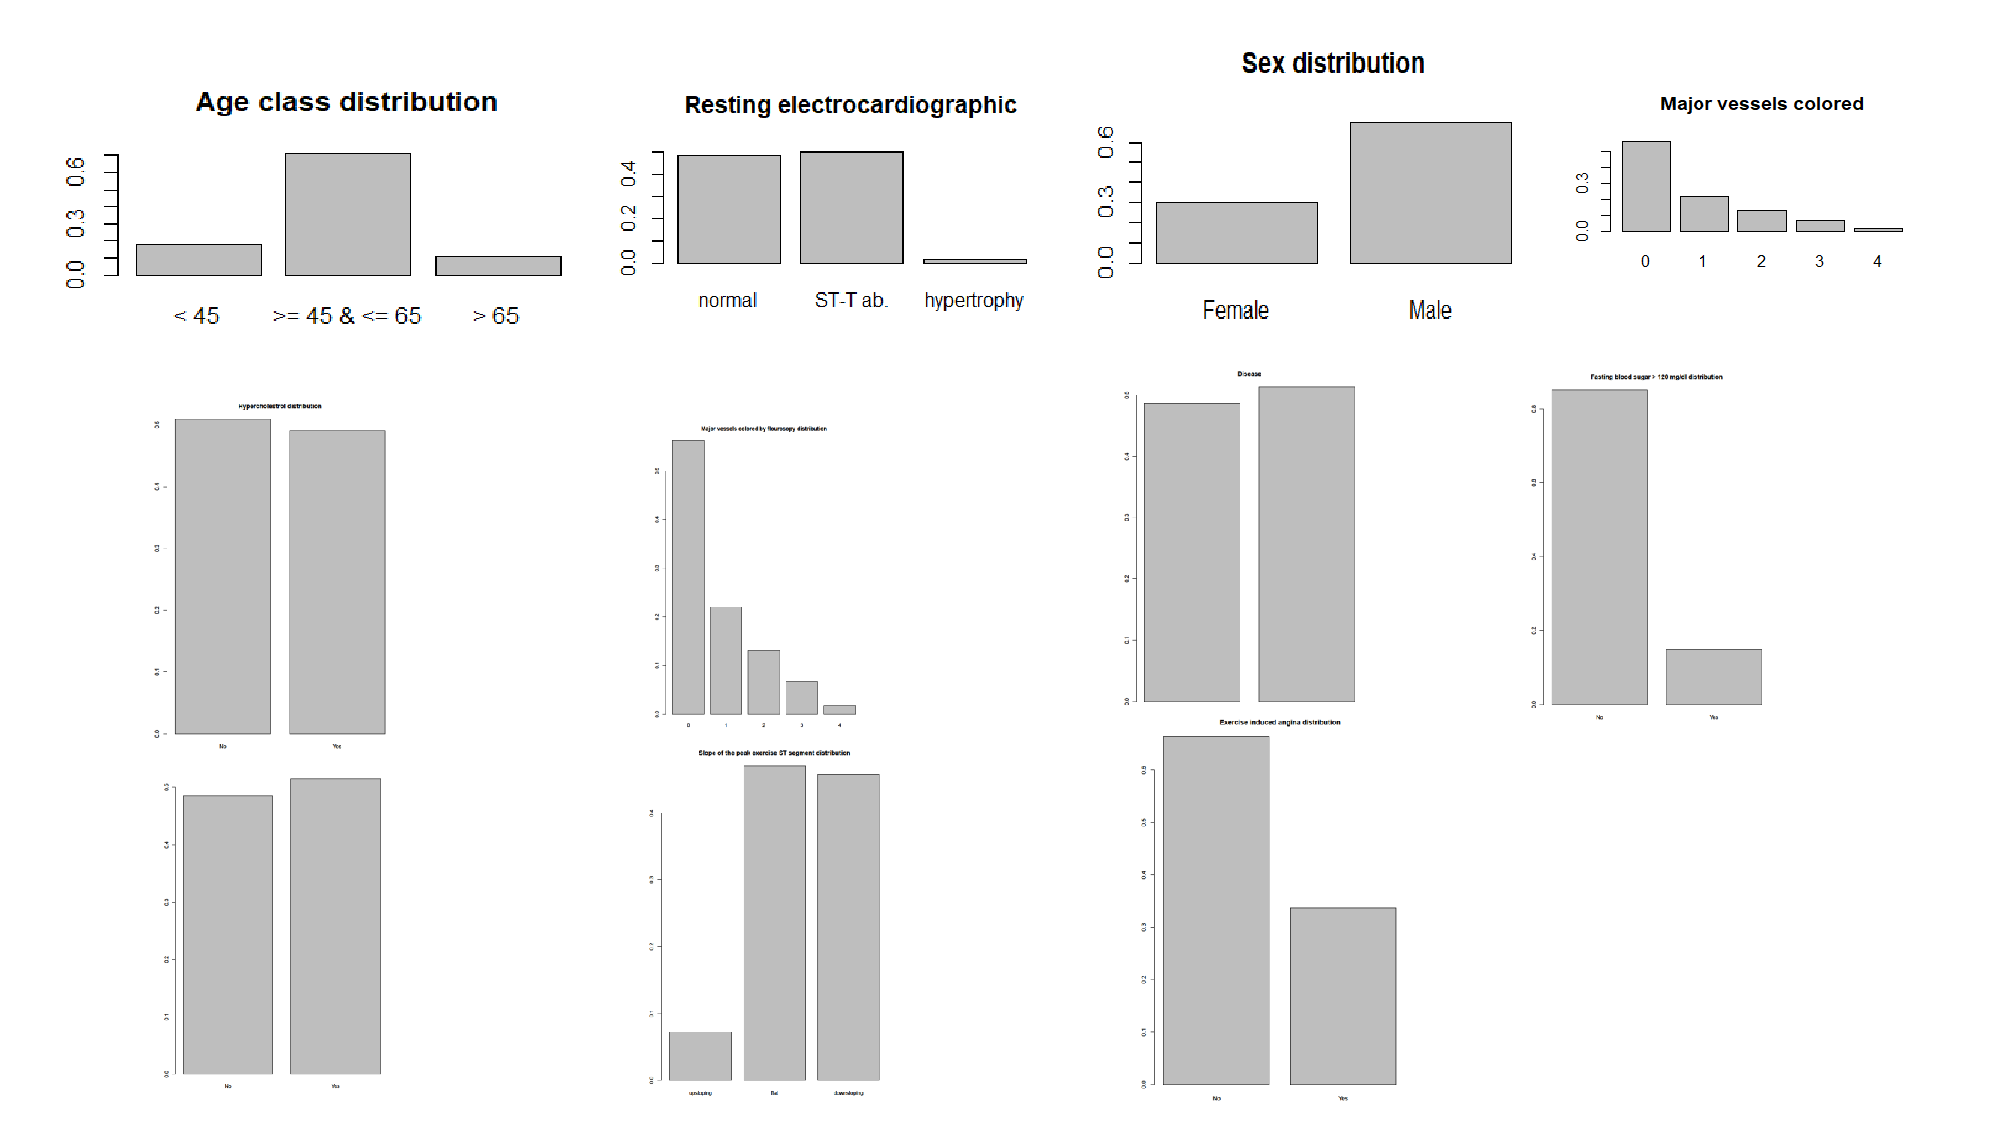
\includegraphics[width=1\textwidth]{plots.pdf}
       \caption{Discrete variables distributions}
   \end{figure}
   
\subsection{Objectives}
The hereby project has two different but related aims: analyze the relationships among the set of discrete variables by the means of log-linear model and undirected graphs to compare the results with those in \cite{Steno}. A more detailed analysis is the carried out considering all variables via bayesian networks and oriented graphs, then the results of the analyses are matched with those in literature.\\

Scientific community has reached a widespread agreement about the main factors that cause heart diseases: high blood pressure, high cholesterol and age are the most relevant factors. However, there is no clear evidence if heart disease and sex are dependent or not. US CDC hints that men and women are affected alike while suggests that it may not be true \cite{Steno} \cite{Health-related variables} \cite{CDC paper}.

\section{Methodology}
To be consistent in the following explanation the notation of \cite{book} and \cite{ArtInt} are used.

\subsection{Log-linear models}
Log-linear models were designed and developed just for categorical and discrete variables to map the log of the probabilities into the sum of interaction factors between variables that are easier to interpret.\\

Let $\Delta$ be discrete set of variables whose cardinality is $d$. An observation (row of the dataset) $i = (i_1,...,i_d) \in \mathcal{I}$ can be seen as a realization of a vector of random variables $X = (X_v)_{v \in \Delta}$ each one with its own \textit{levels} (i.e. elements of the domain).\\
Log-linear models aim to estimate $Pr(X=i) = p(i) \, \forall i \in \mathcal{I}$ under the assumption of independence. The joint probability of $N$ observations can be expressed as
\begin{equation}
p(i^v,v =1,...,N) = \prod\limits_{v=1}^{N}p(i^v) =  \prod\limits_{i \in \mathcal{I}}p(i)^{n(i)}
\end{equation}
where $n(i)$ is the number of cases for which $i^v = i$.
To make the computation and the treatment of the problem much simpler it is possible to express the logarithm of the probability as the sum of some unknown parameters $u$, called \textit{interaction terms}, if $p(i) > 0$. This approach has a clear advantage indeed it is easier to understand the mutual relationship among variables and the interpretation is straightforward. \\
In mathematical terms, for a 2-dimensional example, an observation of the set $\Delta = \{a,b\}$ is $i = (j,k)$. The logarithm of the probability can be factorized as
\begin{equation}
   \log(p(i)) = u + u^a_j  + u^b_k + u^{ab}_{jk} 
\end{equation}
where $u$ is a constant, $ u^a_j$ is the effect of $a$ through the observed value $j$,  $ u^b_k$ is the effect of $b$ through the observed value $k$ and  $u^{ab}_{jk}$ is the effect of the combination of $a$ and $b$. \\
It is also worth noting that this transformation changes the problem into finding the best fit of the interaction terms which is easier to handle with automated means.\\
A further extension of log-linear models are \textit{hierarchical log-linear models}. They are log-linear that satisfy the following property: if an interaction terms is set to 0, then all the higher order interaction terms are also set to 0. The maximal non zero interaction terms are called \textit{generators} of the models indeed just knowing them allows to reconstruct the presence and the absence of all other interaction terms. \\

Log linear models can be exploited to study the dependence, independence and conditional independence relationships among a set of variables since the interaction terms can be seen as arcs connecting the variables they refer to. \\
Independence relationship $\indep$  between two disjoint sets of variables $A$ and $B$ can be expressed in mathematical terms as 
\begin{equation}
    A \indep B  \iff
        \begin{cases}
        \; f(A,B)=f(A)f(B) \\
        \: f(A|B) = f(A) \\
        \; f(B|A) = f(B)\\
        \end{cases}
\end{equation}
where $f$ is the (joint) density function. \\

Conditional independence requires the set of variable $\Delta$ to be divided into at least three disjoint subsets $A$, $B$ and $C$ such that
$X_A=(X_v)_{v \in A}$, $X_B=(X_v)_{ v \in B}$ and $X_C=(X_v)_{ v \in C}$.
$A$ is independent from B given C, i.e. $A \indep B | C$, if 
\begin{equation}
    f(X_A,X_B,X_C) = f(X_A|X_C)f(X_B|X_C)
\end{equation}
or if the factorization criterion
\begin{equation}
    f(X_A,X_B,X_C) = g(X_A,X_C)h(X_B,X_C)
\end{equation} holds. \\

Let $\mathcal{G}$ be an undirected graph $\mathcal{G} = (V,E) $ with cliques $C_1,...,C_k$. If  there exist the factorization
\begin{equation}
    f(X_v) =  \prod\limits_{i=1}^{K}g_i(X_{C_i})
\end{equation} where $g_i$ depends on $X$ only through $X_{C_i}$ then $f$ factorizes accordingly to $\mathcal{G}$ and the model is \textit{graphical}.
If all the densities in the model factorize accordingly to $\mathcal{G}$, then every time $A$ and $B$ are separated by $C$ then $A \indep B | C$ holds.
To make relationships clear the models can effectively and easily be visualized using undirected graphs. Indeed, two independent variables have no arc that connects them if and only if their interaction term is 0; while non zero values are represented as arcs in the graph. \\

\subsection{Model selection}
The model selection can be a very tricky problem, indeed there exist $2^{\frac{(d \times d-1)}{2}} = O(2^{d})$ possible meaningful undirected graphs; for even a small $d = 14$ there are $2^{91}$ possible models. The best model in such a big model space cannot be found defining manually the models and selecting them accordingly to a metric. The best way to proceed is to use fully automated model selection techniques provided by R. Indeed, the R function \textit{stepwise} is used to select the best log-linear model.
It can work in two modalities backward and forward. In backward modality the function uses the saturated model (i.e. the model with all possible arcs) and, at each step, deletes the arc that induces the maximum decrease in a selected metric. On the contrary, the forward mode starts by a null model (i.e. a model without arcs) and, at each step, adds the best possible arc accordingly to the chosen metric. In the end, the metric-minimizing models selected. \\
Two metrics are commonly used to evaluate a model $M$: Akaike information criteria \begin{equation}
   AIC(M) =  -2 \log L(M) + 2r(M) 
\end{equation}
or Bayes information criteria (BIC)
\begin{equation}
   BIC(M) =  -2 \log L(M) + \log(N) r(M) 
\end{equation}
where $r(M)$ is the number of free parameters the model has and $L(M)$ is the likelihood function
\begin{equation}
    L(p) \propto  \prod\limits_{i \in \mathcal{I}}p(i)^{n(i)}
\end{equation}
Notice that there is no need to know the exact value of the likelihood function since we are interested in the ranking of models that is not affected by the presence of constants, hence the proportional symbol ($\propto$). \\
BIC score is more suitable than AIC since it tends to select the simplest model consistent with the data, as it happens for the dataset analyzed.


\subsection{Bayesian networks}
Log-linear models left the reader with two important unanswered questions: how can the continuous variables be exploited? Can directed graphs be exploited to better understand the relationships among variables? \\
Bayesian networks provide the answer to those questions: indeed they can handle both continuous and discrete variable and can be represented by direct acyclic graphs (DAG). \\
Moreover, they can also incorporate some prior knowledge about the domain of the problem; for instance it is possible to prevent arcs from connecting factors to causes, while allowing factors to be connected to effects.\\

A graph $\mathcal{G} = (V,E)$ representing a bayesian network is composed by a set of vertices $V$ and a set of edges $E \subseteq V \times V$ such that 
\begin{enumerate}
    \item Each node $v_i$ corresponds to a random variable of $X_i \in  \Delta$.
    \item A directed arc,  $v_i \rightarrow v_j$ may connect two nodes $v_i$ and $v_j$. If it happens $v_i$ is said to be the parent of $v_j$.
    \item Each node $v_i$ is associated to a conditional probability distribution \\
    $P(v_i  |Parents(v_i))$ that represents the effect of the parents on the node. It is worth noting that the parent of a node can be  a set of continuous nodes or a set of discrete nodes or a combination of the two.
\end{enumerate}
The introduction of directed arcs and thus the ordering between parents and children allows to interpret the parents nodes (or variables) as a set of factors contributing to the realization of the events represented by the children node (variable). However, it is not possible to interpret the arc as a causal relationship\footnote{There exists \textit{causal} bayesian networks to find out causal relationships} without the risk of being wrong.\\

The joint probabilities of a sample $i$ from $X$ can be factorized by using the low of conditional probabilities by traversing backward the net until nodes have no parents. In mathematical terms, the joint probability of $i$ is expressed as
\begin{equation}
    p(v_1 = i_1...,,v_d=i_d) = \prod\limits_{i=1}^{d}p(v_i|Parents(v_i))
\end{equation} \\
As before, the most challenging aspect of bayesian network is how to construct a model from the data. The main problem, again, is that the number of possible network is exponential in the number of variables $O(2^d)$, indeed it is a $NP-Complete$ problem. When facing such problems a brute-force search of the best model is not feasible in finite time even for $d$ not too big, therefore approximated techniques or heuristics to optimize a score should be applied to guide the search. As before the scores that can be applied in the present domain are BIC and AIC.\\
The R library used in the project exploits a simple but efficient greedy algorithm known as hill climbing algorithm (hc). Greedy algorithms are algorithms that follow an heuristic to compute locally optimal choice which may lead to globally optimal solutions, they can be often exploited to solve very hard problem with a reasonable approximation\footnote{Famous greedy algorithms are Prim's, Kruskal's and Dijkstra's}. Hc is a local optimizer that is guaranteed to converge to the global optimum if and only if the optimization problem is convex. It is not a very complex techniques but it can provide good results in reasonable time.
\begin{figure}[H]
       \centering
       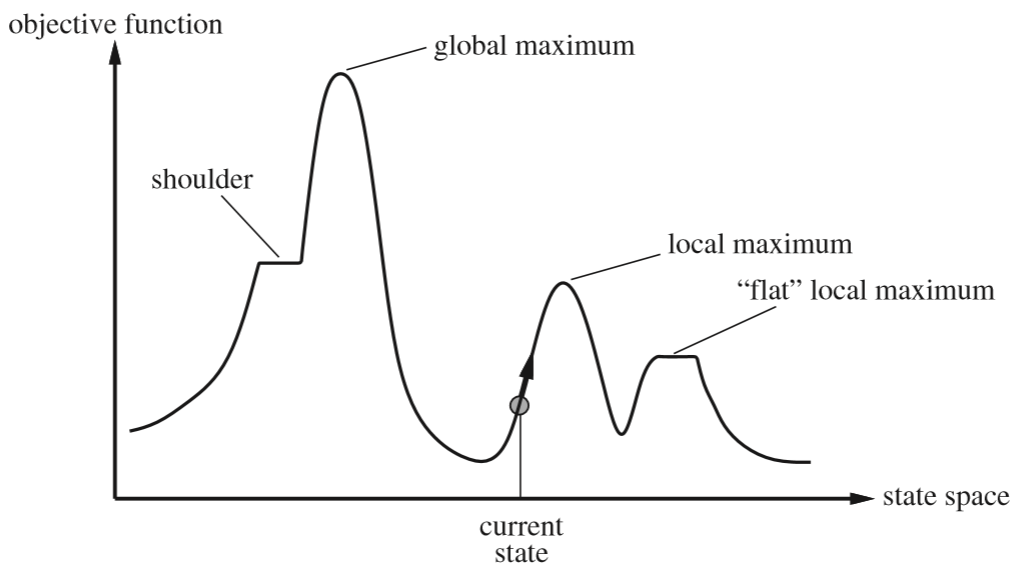
\includegraphics[width=1\textwidth]{hc.PNG}
       \caption{Univariate non convex function optimization problems \cite{ArtInt}}
\end{figure}
However, it may get stuck in a local optimum or shoulder and never find the global optimum as shown in Figure 2. To prevent this from happening a stochastic hill climbing algorithm can be used. The main idea behind stochastic optimization is to move at times to a random point in the state space to search optima near it. It is worth noting that the techniques is not guaranteed to converge to the global optimum but may reach it even if it starts near a local optimum. The following algorithm provides a brief overview of the hill climbing algorithm for discrete and continuous variables.
\begin{algorithm} [H]
   \caption{Hill Climbing}
    \begin{algorithmic}[1]
        \State \textbf{inputs}: 
        \State M1 \Comment{Initial model}
            \State \textbf{initialization:}
            \Do
            \State Evaluate the cost of the current model
            \State Compute the gradient of the continuous variables
     	    \State Compute the best value for discrete variables by scanning the neighbours
     	    \State Evaluate the new model M
 	   \If{M has lower cost that M1}
 				\State M1 = M
 		\EndIf
 		\doWhile{Convergence is not reached} 
 \State \textbf{return}:  M
\end{algorithmic}
\end{algorithm}
As previously stated it is possible to use stochastic search for continuous variables using stochastic gradient descent. While adding stochastic neighbours to the discrete variables is a suitable technique. \\
There are more complex algorithms such as simulated annealing that try to move away from local optima by starting the search from many different points. \\
The model thus created may be compared with model produced by other algorithms or by the information provided by expert to double-check the findings. \\


\section{Results}
\subsection{Log-linear models}
Four log-linear models were investigated to understand the relationship among discrete variables: ``Initial forward model" is the saturated model, ``AIC" is the model generated by the backward search optimizing AIC, ``BIC" by the backward search optimizing BIC score. On the contrary, ``Initial backward model" was created by the forward search from a null model optimizing BIC score.
\begin{figure}[H]
       \centering
       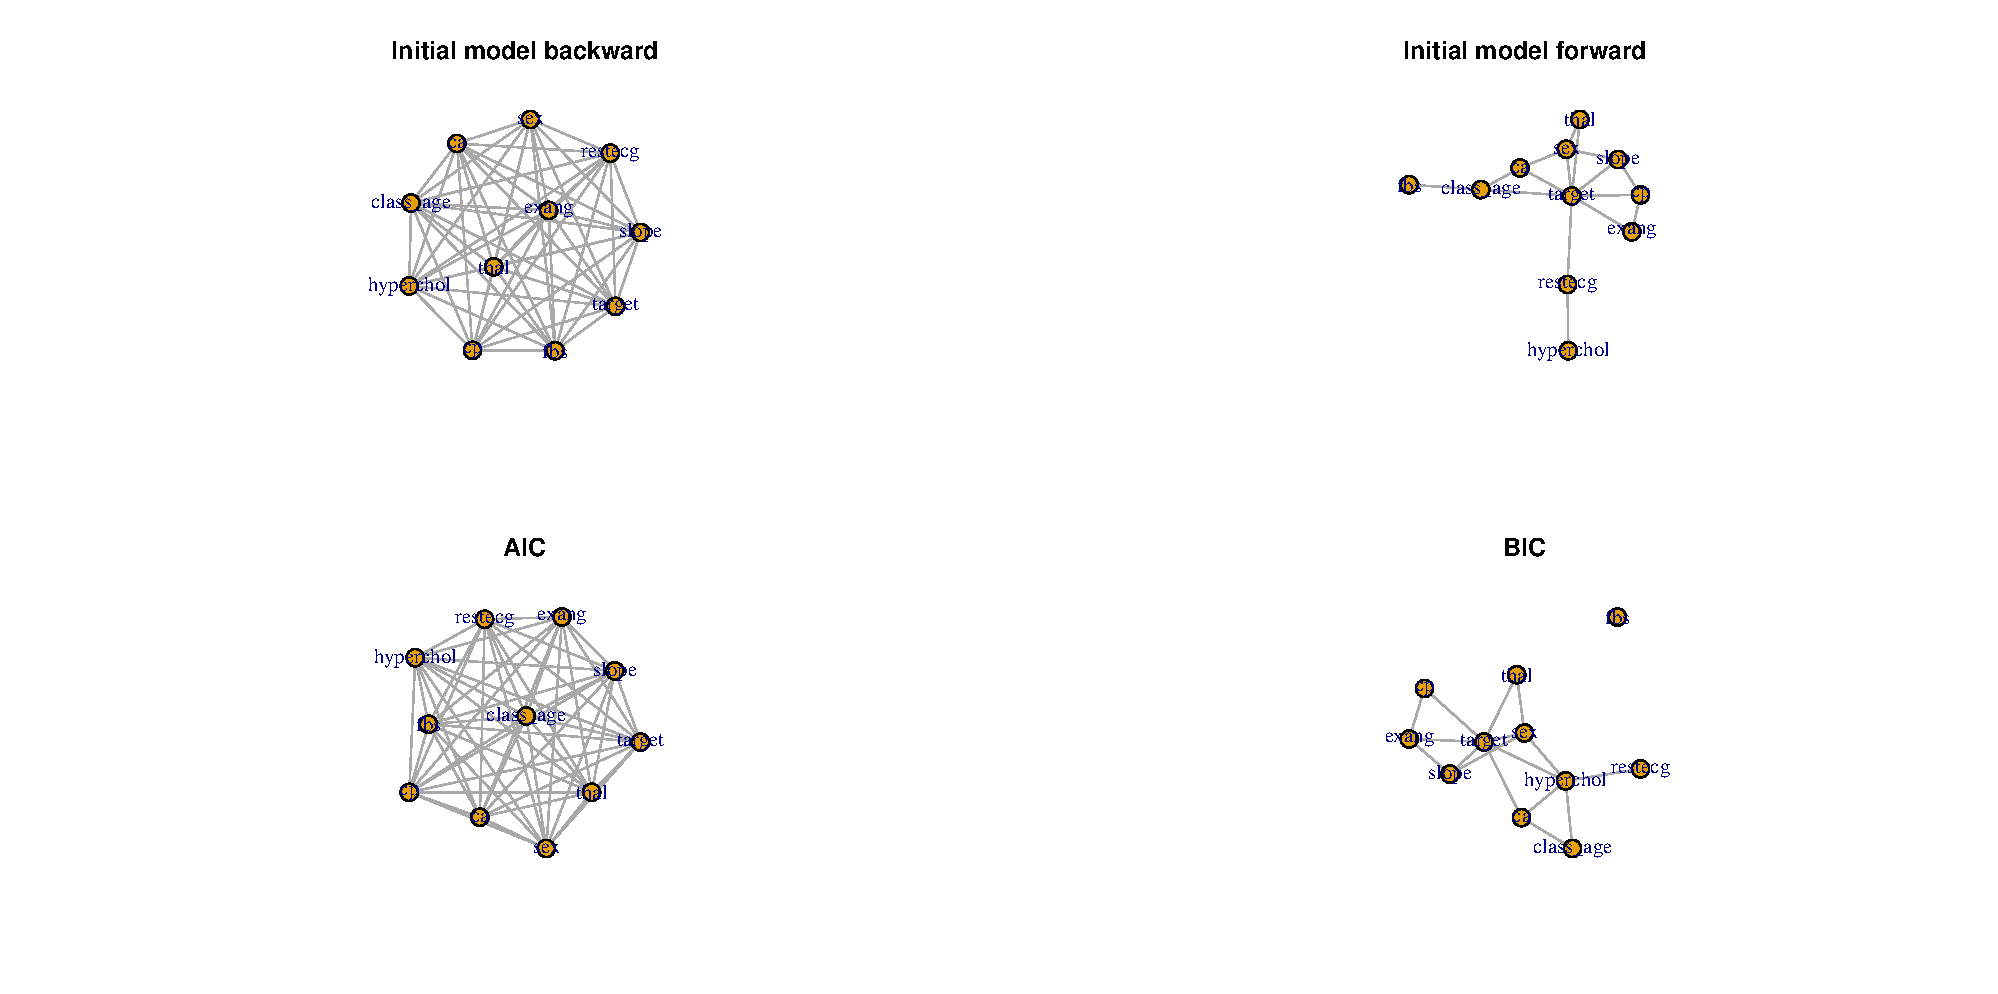
\includegraphics[width=1\textwidth]{Log-linear discrete results.pdf}
       \caption{Log-linear models}
\end{figure}
``Initial forward model" and ``AIC" are useless model since they are represented by fully connected graphs. However, the remaining hierarchical models carry some useful information.
The choice of parsimonious models may be due to both the choice of starting from a null model and to the use of Bayes information criteria. \\

``BIC'' results are consistent with those found in literature but there is only one exception: sex; indeed it is linked to target in all four models. However, the results in literature use much greater amount of  data, therefore the results found may not be as statistically sound as those of CDC.\\
There is only one isolated node \textit{fbs} in ``BIC'' that is connected in all other graphs. This may suggest that the interaction terms referring to it are very weak since I have not found in literature analysis concerning this variable. \\

Some more detailed comparison can be done between ``BIC'' and the model in \cite{Steno}, bearing in mind that they are slightly different: indeed, as can be seen from figure b, heart disease and its symptoms are highly connected and are clustered  in the same node, while in ``BIC'' they are separated nodes; still the result are compatible. More precisely, in both analyses heart disease and sex are dependent as well as hear disease and hypercholesterolemia. Consistent with the result of this project is also the fact that heart disease and ST weaves are dependent.
\begin{figure}[H]
       \centering
       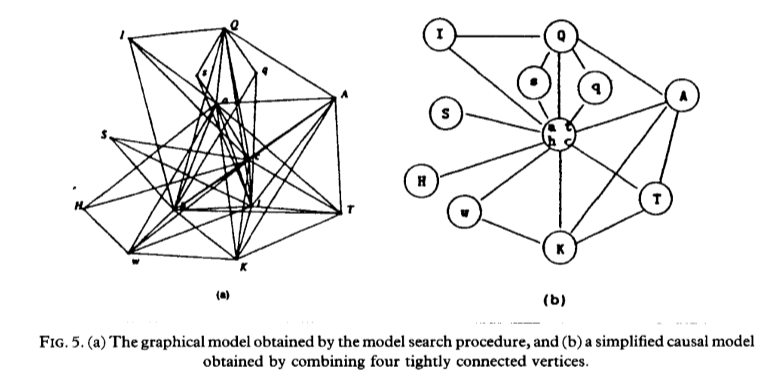
\includegraphics[width=1\textwidth]{Steno graph.PNG}
       \caption{Steno results \cite{Steno}}
\end{figure}

\begin{figure}[H]
       \centering
       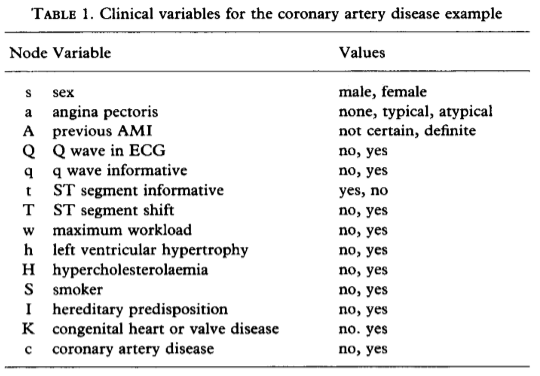
\includegraphics[width=1\textwidth]{steno variables.PNG}
       \caption{Steno variables \cite{Steno}}
\end{figure}

\subsection{Bayesian networks}
The bayesian network build are not guaranteed to be causal bayesian networks, still a good model of the data should resemble the causal structure of reality. To build such a graph some information are added to the model. Variables are divided in four different classes: background variables (1), disease (2), symptoms (3) and measurement of the symptoms (4) where an order relationship holds. There cannot be arc going from a variable in $i$ to a variable in $j$ where $i > j$, which means for instance that symptoms cannot have an arc going to the disease, while clearly a disease can and should be the parent of the symptoms. \\

The model produced by the algorithm exploiting the ordering of the four sets of variable seems to be very precise. Indeed it is able to reconstruct the logical order and the dependence relations between variables. For instance, chest pain influences the slope of the ecg waves and has, as child, its symptom (\textit{exang}). 
Another interesting fact it that \textit{fbs}, as in one of the previous models, does not depend on background variables and disease.
Also thalach seems not to be a very interesting variable indeed, even if it is a background variable it has no children. \\
The model computed seems able to detect the factor influencing the heart disease which are blood pressure (\textit{thal}) and cholesterol (\textit{hyperchol}). It is worth noting that in this model age is independent from the disease which is not consistent with CDC results. However, the model correctly represents the conditional independence of sex and disease given hypercholestroelmia and blod pressure.\\

The following graph represents all the relationships described as well as the bayesian network extracted from the data
\begin{figure}[H]
       \centering
       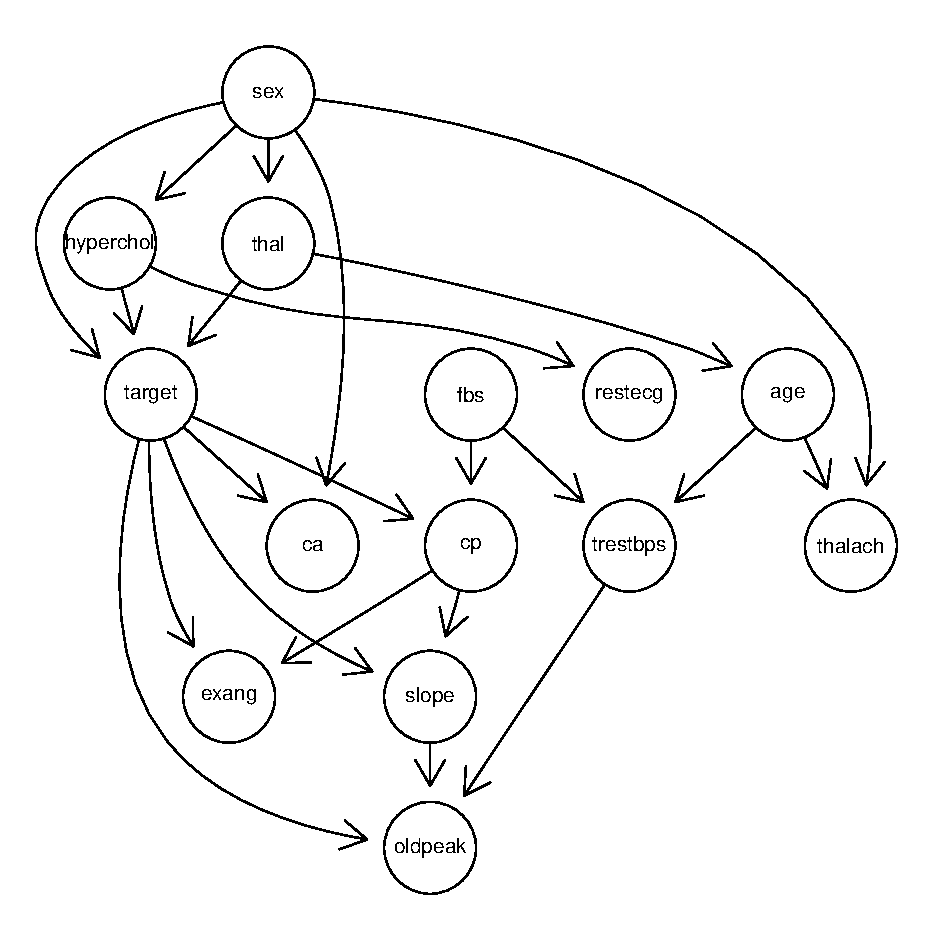
\includegraphics[width=1\textwidth]{bn res.pdf}
       \caption{Bayesian network}
\end{figure}


\section{Conclusions}
Overall, the models are able to detect the two most important factors that contribute to heart disease, blood pressure and hypercholesterolemia, accordingly to the literature. In particular, bayesian network combined with prior information produce the most interesting, accurate and relevant results.\\
The role of sex and age changes with the model and it is not consistent with the literature. This may come from the dataset which might be biased or not as big as those of CDC and other important research institutions.


\newpage

\section{Appendix: Code}
\begin{verbatim}
# Import libraries
library(Rgraphviz)
library(igraph)
library(gRbase)
library(gRim)
library(bnlearn)
library(DAAG)
library(lattice)
library(ggm) 


# Read the dataset
setwd("C:/Users/simon/Desktop/Graphical Model/probabilistic_modelling")
data <- read.csv(file = 'heart.csv')
data <- data[c(14,1,2,3,4,5,6,7,8,9,10,11,12,13)]

data$target <- factor(data$target)
data$sex <- factor(data$sex)

data$cp[data$cp>= 1] <- 1
data$cp[data$cp < 1]  <- 0
data$cp <- factor(data$cp)

data$fbs <- factor(data$fbs)

data$restecg <- factor(data$restecg)

data$exang <- factor(data$exang)

data$slope <- factor(data$slope)

data$ca <- factor(data$ca)

data$hyperchol <- data$chol
data$hyperchol[data$hyperchol<= 240 ]  <- 0
data$hyperchol[data$hyperchol> 240]  <- 1
data$hyperchol <- factor(data$hyperchol)

data$thal <- factor(data$thal)

data$class_age <- data$age

data$class_age[data$class_age<45] <- 1
data$class_age[ data$class_age>=45 & data$class_age<=65] <- 2
data$class_age[data$class_age>65] <- 3
data$age <- as.double(data$age)

data$trestbps <- as.double(data$trestbps)

data$chol <- as.double(data$chol)

data$thalach <- as.double(data$thalach)

data$oldpeak <- as.double(data$oldpeak)

head(data)


# Analysis of the distributions of discrete  variables
barplot(prop.table(table(data$target)),
        main="Disease",names.arg=c("No", "Yes") )
        
barplot(prop.table(table(data$sex)), 
        main="Sex distribution",  
        names.arg=c("Female", "Male"))
        
barplot(prop.table(table(data$cp)),
        main="Chest pain distribution",  
        names.arg=c("No", "Yes"))
        
barplot(prop.table(table(data$fbs)), 
        main="Fasting blood sugar > 120 mg/dl distribution",  
        names.arg=c("No", "Yes"))
        
barplot(prop.table(table(data$restecg)), 
        main="Resting electrocardiographic",  
        names.arg=c("normal", "ST-T ab.","hypertrophy"))
        
barplot(prop.table(table(data$exang)), 
        main="Exercise induced angina",  
        names.arg=c("No", "Yes"))
        
barplot(prop.table(table(data$slope)),
        main="Slope of the peak",  
        names.arg=c("upsloping", "flat","downsloping"))
        
barplot(prop.table(table(data$ca)), 
        main="Major vessels colored")
        
barplot(prop.table(table(data$thal)), 
        main="Thal distribution")
        
barplot(prop.table(table(data$hyperchol)), 
        main="Hypercholestrol distribution",  
        names.arg=c("No", "Yes"))
        
barplot(prop.table(table(data$class_age)),
        main="Age class distribution", 
        names.arg=c("< 45", ">= 45 & <= 65", "> 65") )


data_table <- as.table(ftable(data[c(1,3,4,7,8,10,12,13,14,15,16)]))

# Log linear models
m_sat <- dmod(~.^.,data=data_table) 
m1 <- stepwise(m_sat)
m2 <- stepwise(m_sat,k=log(sum(data_table)))
m3  <- stepwise(dmod(~.^1,data=data_table) ,k=log(sum(data_table)),direction="forward",details=1)


igraph.to.graphNEL(as(m_sat,"igraph"))
igraph.to.graphNEL(as(m1,"igraph"))
igraph.to.graphNEL(as(m2,"igraph"))
igraph.to.graphNEL(as(m3,"igraph"))

m3
summary(m3)
m2
summary(m2)

x11()
par(mfrow=c(2,2))
plot(as(m_sat,"igraph"),main="Initial model backward")
plot(as(m3,"igraph"),main="Initial model forward")
plot(as(m1,"igraph"), main="AIC")
plot(as(m2,"igraph"), main="BIC")

#Bayesian network

bn_data = data[c(1,2,3,4,5,15,7,8,9,10,11,12,13,14)]
classes <- c(2,1,1,3,4,1,1,1,1,3,4,4,4,1)
FrobiddenArcs <- matrix(0, nrow=length(bn_data), ncol=length(bn_data)) 
rownames(FrobiddenArcs)  <- names(bn_data) 
colnames(FrobiddenArcs) <- names(bn_data)
for (b in 2:4){
        FrobiddenArcs[classes==b, classes<b] <- 1 
}

ForbiddenList <- data.frame(get.edgelist(as(FrobiddenArcs, "igraph")))
names(ForbiddenList) <- c("from", "to") 
bn_model <- hc(bn_data, blacklist=ForbiddenList)
x11()
plot(as(amat(bn_model), "graphNEL"))


\end{verbatim}

\newpage
\begin{thebibliography}{9}

\bibitem{dataset}
\textit{https://www.kaggle.com/johnsmith88/heart-disease-dataset}

\bibitem{original_dataset}
\textit{https://archive.ics.uci.edu/ml/datasets/heart+Disease}

\bibitem{Steno}
\textit{STENO: an expert system for medical diagnosis based on graphical models and model search} Lars Rude Andersen, Jens Herman Krebs, Jens Damgaard Andersen, University of Copenhagen Published online: 28 Jul 2006.

\bibitem{book}
\textit{Graphical Models with R}
Authors: Højsgaard, Søren, Edwards, David, Lauritzen, Steffen. 2012.


\bibitem{ArtInt}
\textit{ Artificial Intelligence: A Modern Approach}  Stuart J. Russell, Peter Norvig.


\bibitem{Health-related variables}
\textit{Health-related variables and predictors of Health-promoting Lifestyle in cardiovascular disease patients} Hossein Mohsenipouya, Fereshteh Majlessi, Davood Shojaeizadeh, AbbasRahimi Foroushani,Rahman Ghafari, Vali Habibi,Azam Seyfi Makrani.

\bibitem{CDC paper}
\textit{Prevalence of Uncontrolled Risk Factors for  Cardiovascular Disease: United States}, 1999–2010, Cheryl D. Fryar, Te-Ching Chen, Xianfen Li.

\end{thebibliography} 
\end{document}